\subsection{Illustrative example: Certification and Design Transclusion }
\begin{figure}[ht]
	\centering 
	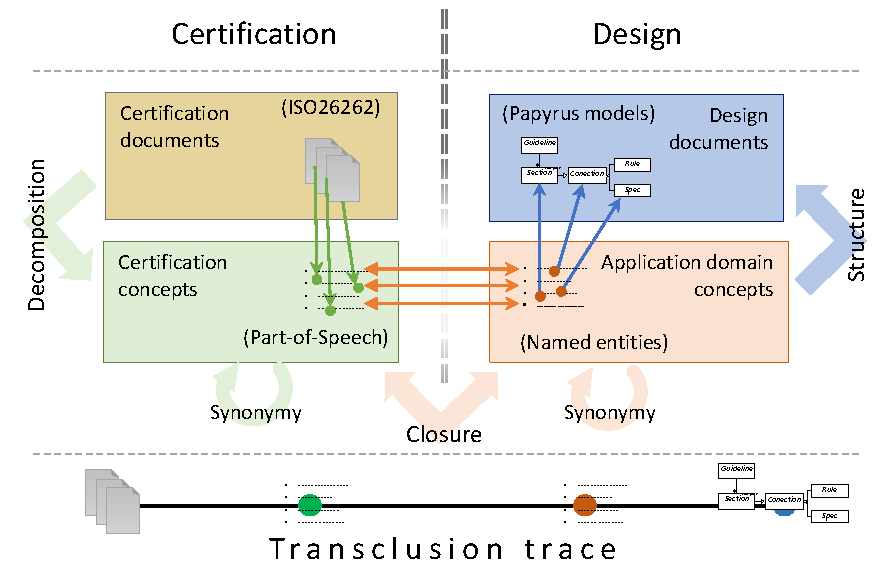
\includegraphics[width=.85\linewidth]{images/metamodel-re}
	\caption{Transclusion of part-of-speech to model entities.}
	\label{fig:metamodel-re}
\end{figure}
 
Certification documents are external to the software system they are certifying. This means that when the software evolves, the content of these documents must be reevaluated to see if the new version of the system can still satisfies the certification conditions. Ideally we would only like to examine the certificate against the changes. And similarly for any change in the certification rules or conditions. We would like that only those parts of the system potentially being affected need to be reviewed and adapted if necessary. 
To be able to support this ``incremental'' evaluations and facilitate the  co-evolution of certification and design artefacts, we need to keep track of the links between the nominal expressions in certifications documents and the elements of design models they target or impact. 
 
As can be seen on the certification side in Figure \ref{fig:metamodel-re}, nominal expressions form semantically rich patterns (\textit{e.g.,} nominal groups, action verbs, nouns, acronyms). They are spread among the sections of the certification documents. The patterns of Parts-of-Speech (PoS) can be extracted using natural language processing  techniques\footnote{The quality of PoSs vary depending on the technique used, its parameterization, as well as the dataset used for training. These choices remain mostly arbitrary and evidences of the superiority of one algorithm or method upon the others remain haphazard~\cite{zou2010-term-based-enhancement-for-trace-retrieval}. In this report, we aim at conceptualizing the problem domain, we do not provide details on the choice and parameterization of such techniques.} 
%\ugh{Maybe ref to annexes with Figure "Linking PLM (decisions) to Papyrus (implementation)" from September CEA meeting.}  

On the design side, named entities are model entities characterized by a unique name (\textit{e.g.,} a method, a class, a package, a model). The structural hierarchy represented by Papyrus models can be used to cluster and disambiguate its constitutive entities~\cite{patel2015-hierarchical-clustering}.
Named entities have synonyms that must be considered as well - and disambiguated when possible.
The association between PoSs and model entities is established with a neural model capable of measuring the (semantic) distance between the elements of both realms\footnote{An interesting methodology to do so is to train a "general intelligence", or to "generally train" a model from available vast corpuses in (more or less) natural language. Then this model is refined with corpuses relevant to the application domain the system belongs to~\cite{shen2015-linking-entities-with-knowledge-base}.}. 
\\
Certification documents are semi-structured text artefacts. Their implementation and validation scenarios may correlate in many different ways with their corresponding modelling entities. We chose the most straight forward case to illustrate an application of the Tracea metamodel: the transclusion of \texttt{PoS} to \texttt{NamedEntities}. Figure \ref{fig:metamodel-re} shows a high level representation of a this process.

This example helps grasp the details of the application of our traceability language to a specific domain: 
%the transclusion of parts of speech in certification documents with their corresponding model elements in Papyrus models. 
an explicit record of the link between important elements of certification and the entities they target in Papyrus models to allow direct transclusion\footnote{A transclusion is the inclusion of part or all of a document into one or more other documents by hypertext reference.}.

Transclusion traces use vertical links (from documents to PoS, and from model to named entity), and horizontal links (between the synonyms and the closure between PoSs and named entities). 
Links related to the composition are explicit: they are contained in the syntax of the domain (\textit{e.g.,} classes are \textit{part} of a package); whereas synonyms and closure are implicit (\textit{i.e.,} they do not appear in the syntax).
This example has a post-requirement nature as it is established after the requirements have been determined.
